\documentclass[aspectratio=169,xcolor=pdftex,dvipsnames,table]{beamer}\usepackage[]{graphicx}\usepackage[]{xcolor}
% maxwidth is the original width if it is less than linewidth
% otherwise use linewidth (to make sure the graphics do not exceed the margin)
\makeatletter
\def\maxwidth{ %
  \ifdim\Gin@nat@width>\linewidth
    \linewidth
  \else
    \Gin@nat@width
  \fi
}
\makeatother

\definecolor{fgcolor}{rgb}{0.345, 0.345, 0.345}
\newcommand{\hlnum}[1]{\textcolor[rgb]{0.686,0.059,0.569}{#1}}%
\newcommand{\hlsng}[1]{\textcolor[rgb]{0.192,0.494,0.8}{#1}}%
\newcommand{\hlcom}[1]{\textcolor[rgb]{0.678,0.584,0.686}{\textit{#1}}}%
\newcommand{\hlopt}[1]{\textcolor[rgb]{0,0,0}{#1}}%
\newcommand{\hldef}[1]{\textcolor[rgb]{0.345,0.345,0.345}{#1}}%
\newcommand{\hlkwa}[1]{\textcolor[rgb]{0.161,0.373,0.58}{\textbf{#1}}}%
\newcommand{\hlkwb}[1]{\textcolor[rgb]{0.69,0.353,0.396}{#1}}%
\newcommand{\hlkwc}[1]{\textcolor[rgb]{0.333,0.667,0.333}{#1}}%
\newcommand{\hlkwd}[1]{\textcolor[rgb]{0.737,0.353,0.396}{\textbf{#1}}}%
\let\hlipl\hlkwb

\usepackage{framed}
\makeatletter
\newenvironment{kframe}{%
 \def\at@end@of@kframe{}%
 \ifinner\ifhmode%
  \def\at@end@of@kframe{\end{minipage}}%
  \begin{minipage}{\columnwidth}%
 \fi\fi%
 \def\FrameCommand##1{\hskip\@totalleftmargin \hskip-\fboxsep
 \colorbox{shadecolor}{##1}\hskip-\fboxsep
     % There is no \\@totalrightmargin, so:
     \hskip-\linewidth \hskip-\@totalleftmargin \hskip\columnwidth}%
 \MakeFramed {\advance\hsize-\width
   \@totalleftmargin\z@ \linewidth\hsize
   \@setminipage}}%
 {\par\unskip\endMakeFramed%
 \at@end@of@kframe}
\makeatother

\definecolor{shadecolor}{rgb}{.97, .97, .97}
\definecolor{messagecolor}{rgb}{0, 0, 0}
\definecolor{warningcolor}{rgb}{1, 0, 1}
\definecolor{errorcolor}{rgb}{1, 0, 0}
\newenvironment{knitrout}{}{} % an empty environment to be redefined in TeX

\usepackage{alltt}
% \documentclass[notes,aspectratio=169,xcolor=pdftex,dvipsnames,table]{beamer}

%\setbeameroption{show notes}

\usepackage{bm,graphicx,amsmath,tikz} %fancybox,
\usepackage{color}%,textpos}
\usepackage[round]{natbib}
\usepackage[normalem]{ulem}
\usepackage{hyperref}
\usepackage{lastpage}
\usepackage{array}
\usepackage{color}
\usepackage{framed}

% Define Western colours
\definecolor{western}{rgb}{.306,.152,.524}
\definecolor{westerngray}{rgb}{.512,.508,.524}

%% Define BEAMER colours
\setbeamercolor{frametitle}{bg=western,fg=white}
\setbeamercolor{framesubtitle}{bg=western,fg=black}
\setbeamercolor{title}{fg=white,bg=western}
\setbeamercolor{author}{fg=white,bg=western}
\setbeamercolor{institute}{fg=white,bg=western}
\setbeamercolor{date}{fg=white,bg=western}

%% Set BEAMER fonts
\setbeamerfont{title}{shape=\bf}
\setbeamerfont{frametitle}{shape=\sc,size=\Large}
\setbeamerfont{framesubtitle}{shape=\sc,size=\Large}
\setbeamerfont{footline}{shape=\sc}

%% Define BEAMER toc
\setbeamercolor{section in toc}{fg=western}
\setbeamercolor{subsection in toc}{fg=westerngray}
\setbeamertemplate{sections/subsections in toc}[ball]

%% Define BEAMER background
\setbeamercolor{background canvas}{bg=white}

%% Define BEAMER footer
\setbeamertemplate{navigation symbols}{}
\setbeamercolor{footline}{fg=white,bg=western}
\setbeamertemplate{footline}{%
  \begin{beamercolorbox}[wd=\paperwidth]{footline}
    \vskip5pt

    \hspace{.1in}
    \raisebox{.05in}{
      \scriptsize{\bf \insertshorttitle }
    }
    \hfill
    \raisebox{.05in}{
      \scriptsize{\bf \insertframenumber/\inserttotalframenumber}
    }
    \hspace{5pt}

    \vskip5pt
  \end{beamercolorbox}
}

%% Define BLOCK environment
\setbeamercolor{block title}{fg=western}
\setbeamerfont{block title}{series=\bfseries}

%% Define ENUMERATE and ITEMIZE environements
\setbeamertemplate{itemize item}[ball]
\setbeamertemplate{enumerate item}[ball]
\setbeamercolor{item projected}{bg=western}

%% Define BEAMER toc
\setbeamercolor{sections/subsections in toc}{fg=blue!75}
\setbeamertemplate{sections/subsections in toc}[ball]

%% Define SECTION openings
\AtBeginSection[]{
}

\title[SS2857 -- Lecture 4]{SS2857 Probability and Statistics 1\\
  Fall 2024\\
  \vspace{.2in}
  Lecture 4}
  
\date{}




\IfFileExists{upquote.sty}{\usepackage{upquote}}{}
\begin{document}

{
\setbeamertemplate{footline}{}
\setbeamercolor{background canvas}{bg=western}

\begin{frame}
  \maketitle
\end{frame}
}

\begin{frame}
  \begin{center}
    \Large{\textbf{2.4 Conditional Probability}}

    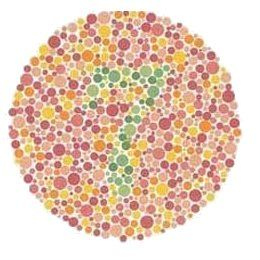
\includegraphics[height = .6\textheight]{colorblind-test-image1.jpg}
  \end{center}
\end{frame}

\begin{frame}{Conditional Probability}
  For any two events $A$ and $B$ with $P(B)>0$, the conditional probability of $A$ given that $B$ has occurred is defined by
  \[
    P(A|B)=\frac{P(A \cap B)}{P(B)}.
  \]
\end{frame}

\begin{frame}{Conditional Probability}

Conditional probabilities essentially reduce the sample space from $\mathcal S$ to some event $B \subset \mathcal S$.

\begin{center}
\only<1>{
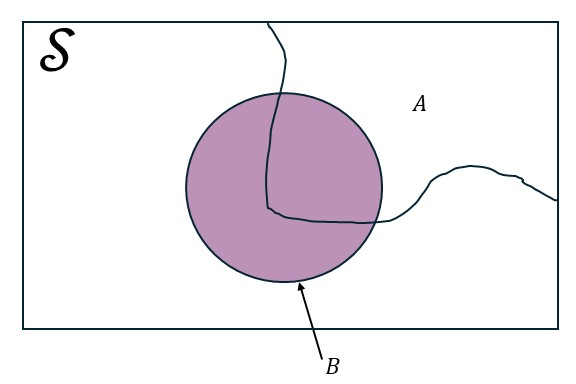
\includegraphics[width=.6\textwidth]{Figures/lecture_4_figures/Slide1}
}
\only<2>{
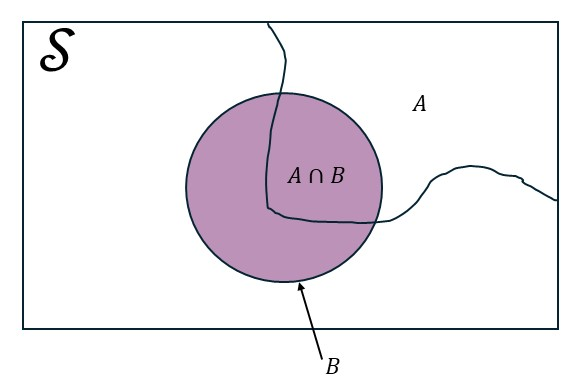
\includegraphics[width=.6\textwidth]{Figures/lecture_4_figures/Slide2}
}
\end{center}
\end{frame}

\begin{frame}{Multiplication Rule}

The multiplication rule is simply a rearrangement of the definition of conditional probability. 

If
  \[
    P(A|B)=\frac{P(A \cap B)}{P(B)}.
  \]
then
  \[
    P(A \cap B)=P(A|B){P(B)}.
  \]

\end{frame}

\begin{frame}
  \begin{block}{Example 4.1}
    According to \url{http://https://www.colourblindawareness.org/}, colour blindness affects 1 in 12 people assigned to be male at birth and 1 in 200 people assigned to be female at birth. Approximately 48.78\% of all babies born in the world are assigned to be female at birth.

    \begin{enumerate}[a)]
      
    \item Identify the conditional probability(ies) in this statement and define them in terms of the events $F$ a person is assigned to be female at birth and $B$ a person is colour blind.
      
    \item What is the probability that a randomly selected newborn is female and colour blind/male and colour blind?
    
    \item What is the probability that a randomly selected newborn is colour blind?
      
    \end{enumerate}
  \end{block}
\end{frame}


\begin{frame}{Law of Total Probability}
  Let $A_1,\ldots,A_k$ be exhaustive,
  \begin{itemize}
  \item mutually exclusive: $A_i \cap A_j=\emptyset$ for all $i,j=1,\ldots,k$, and
  \item exhaustive: $\cup_{i=1}^k A_i = \mathcal S$,
  \end{itemize}
  Then for any other event $B$
  \[
    P(B)=\sum_{i=1}^k P(B|A_i)P(A_i)\left(=\sum_{i=1}^k P(A_i \cap B)\right).
  \]
  
  \medskip
  
  Note: We can also say that $A_1,\ldots,A_k$ partition $\mathcal S$.

\end{frame}

\begin{frame}{Law of Total Probability}
  The law of total probability allows us to compute the probability of an event by summing the probabilities of individual pieces:
  
  \begin{center}
\only<1>{
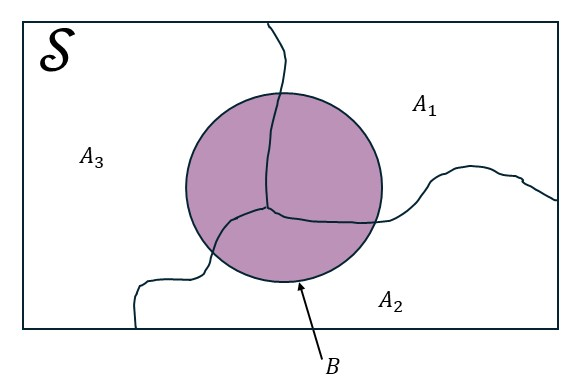
\includegraphics[width=.6\textwidth]{Figures/lecture_4_figures/Slide3}
}
\only<2>{
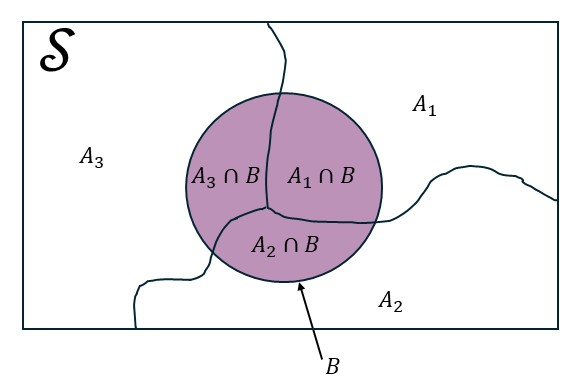
\includegraphics[width=.6\textwidth]{Figures/lecture_4_figures/Slide4}
}
\end{center}

\end{frame}

\begin{frame}
  \begin{block}{Example 4.1}
    According to \url{http://https://www.colourblindawareness.org/}, colour blindness affects 1 in 12 people assigned to be male at birth and 1 in 200 people assigned to be female at birth. Approximately 48.78\% of all babies born in the world are assigned to be female at birth.

    \begin{enumerate}[d)]
      
    \item What is the probability that a baby is assigned to be male at birth given that it is colour blind?
      
    \end{enumerate}
  \end{block}
\end{frame}

\begin{frame}{Bayes' Rule}
  Let $A_1,\ldots,A_k$ be a collection of mutually exclusive and exhaustive events (i.e., a partition of $\mathcal S$) with $P(A_i)>0$ for $i=1,\ldots,k$. Then for any other event $B$ for which $P(B)>0$,
  \[
    P(A_j|B)=\frac{P(B|A_j)P(A_j)}{P(B)}=\frac{P(B|A_j)P(A_j)}{\sum_{i=1}^kP(B|A_j)P(A_j)} \quad j=1,\ldots,k.
  \]
\end{frame}

\begin{frame}{Bayes' Rule}
  Bayes' rule allows us to switch the direction of conditional probabilities so that we can compute the probability of $A_j|B$ from the probability of $B|A_j$:
  \[
    P(A|B)=\frac{P(B|A)P(A)}{P(B)}.
  \]

\end{frame}

\begin{frame}
  \begin{block}{Example 4.1}
    According to \url{http://https://www.colourblindawareness.org/}, colour blindness affects 1 in 12 people assigned to be male at birth and 1 in 200 people assigned to be female at birth. Approximately 48.78\% of all babies born in the world are assigned to be female at birth.

    \begin{enumerate}[e)]
      
    \item What is the probability that someone answers yes to the following statement:\\
      \begin{center}
        I am colour blind \textbf{OR\footnote{We will always use the inclusive or so that the statement is true if one or both are true.}} my birthday falls on an odd numbered day of the month. 
      \end{center}
      
    \end{enumerate}
  \end{block}
\end{frame}

\begin{frame}
  \begin{center}
    \Large{\textbf{Questions?}}
  \end{center}
\end{frame}

\begin{frame}{Exercise 4.1}
The 2024 US Presidential election will be held on November 5 and provides a lot of opportunity for interesting statistics. Current polls put Kamala Harris in the lead nationally with 48\% of the vote versus Donald Trump's 46\% (the remaining 6\% are undecided or voting for other candidates). However, Kamala's support by state varies from 28\% in Utah (population 3,417,734) to 70\% in Vermont (population 647,464). The total population of the 50 US states is 334,235,923. 

\begin{enumerate}[a)]
\item Identify the conditional probabilities defined in this question.

\item What is the probability that a randomly selected US voter is from Utah and is planning to vote for Kamala Harris?

\item What is the probability that someone not from Utah plans to vote for Kamala Harris?

\item Suppose that a randomly selected person is planning to vote for Kamala Harris. Is this person more likely to be from Utah or from Vermont? 

\item What is the key assumption to answering these questions?
\end{enumerate}

\end{frame}

\end{document}
